%! Author = Administrator
%! Date = 2021/7/2

\chapter{系统测试与分析}
基于测试驱动开发的思想,在本章提出了交付的指标要求和具体测试方式,对整个系统的功能性、稳定性、并发性、可用性等多维度进行评价,确保该
系统改进的有效性,是否可以满足预期结果

\section{测试环境和工具}

\subsection{测试硬件环境}
云服务器一台
4核 / 4GB内存
容器镜像Centos7

\subsection{测试工具和方法}

\begin{figure}[H]
    \centering
    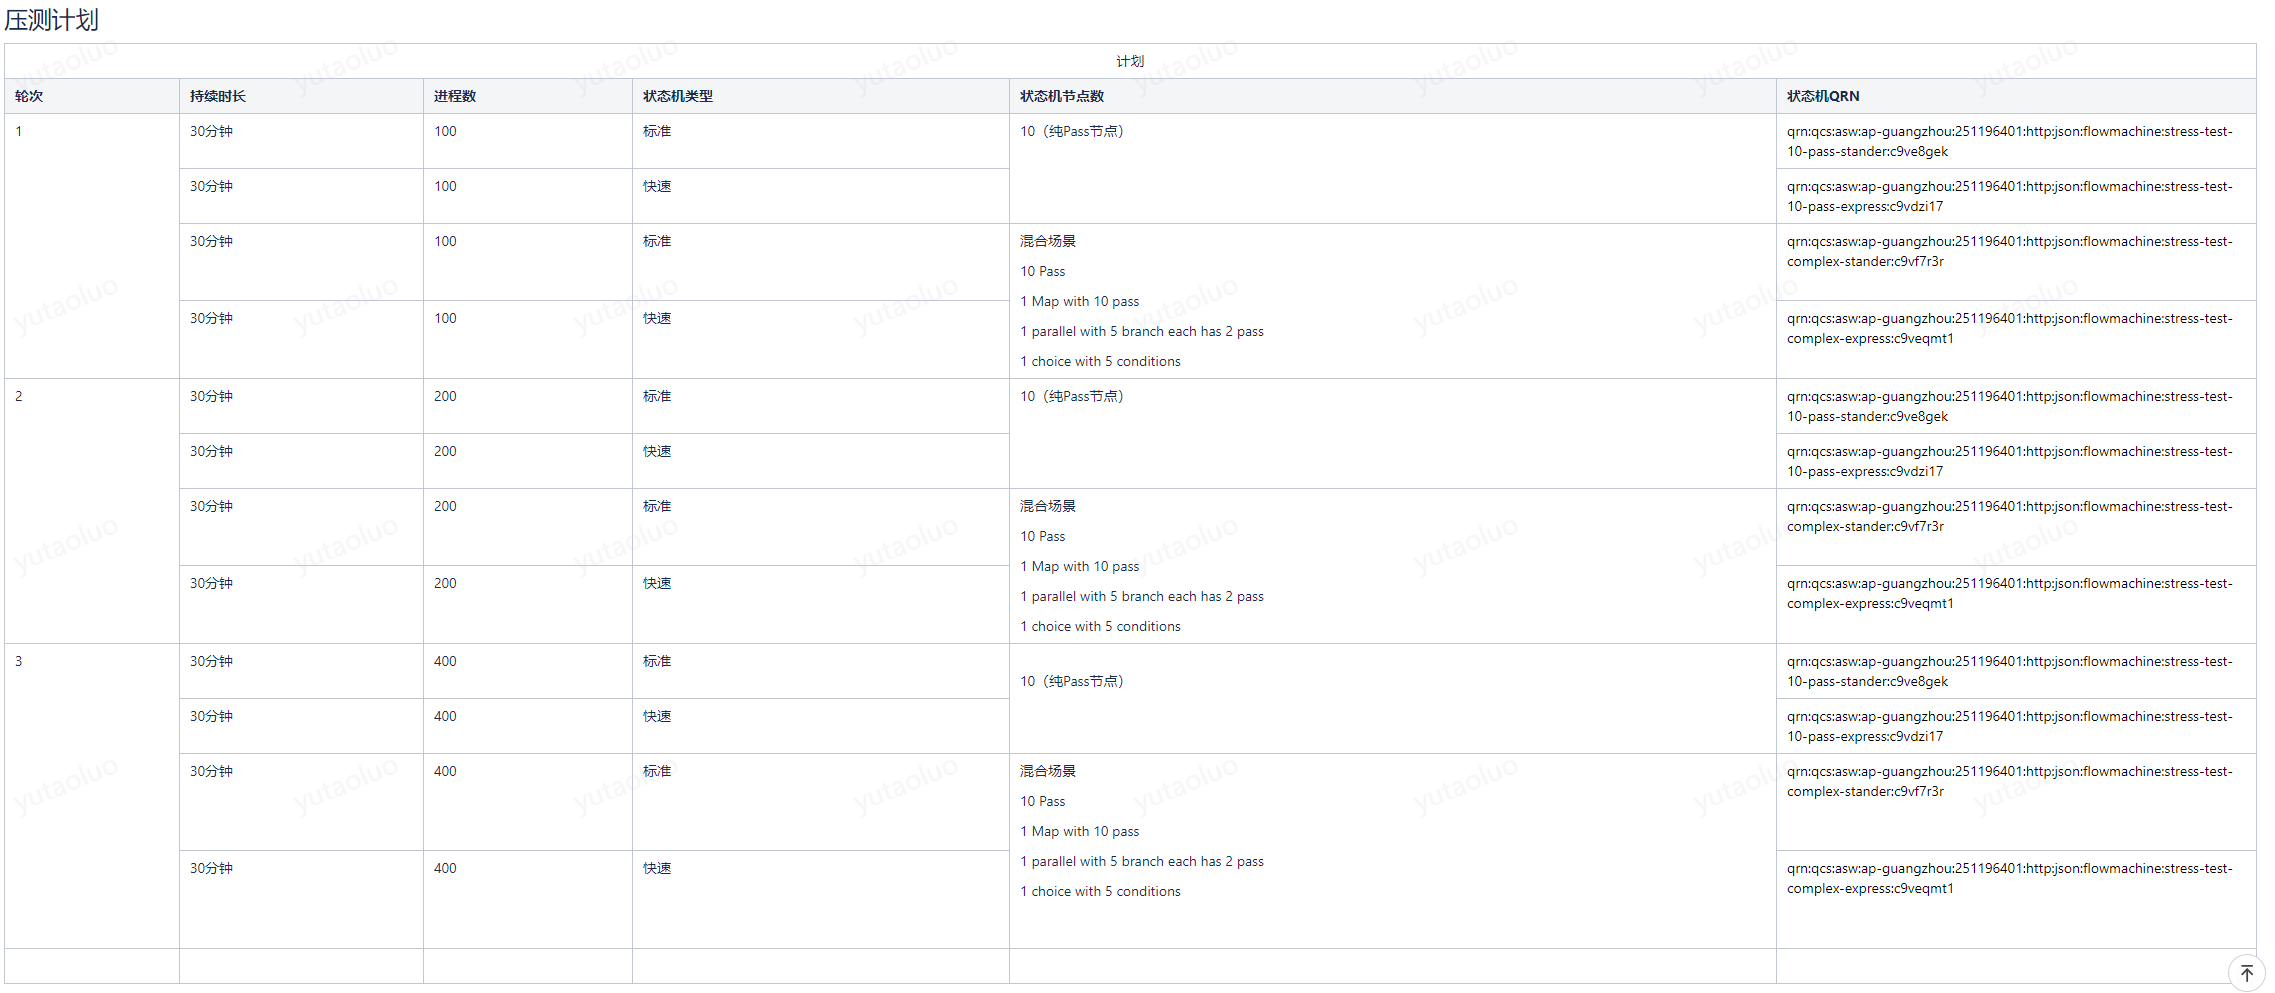
\includegraphics[width=0.9\textwidth]{press-test-1.png}
    \caption{6-3-1}
    \label{fig:6-1-1}
    \note{压测计划1}
\end{figure}

\begin{figure}[H]
    \centering
    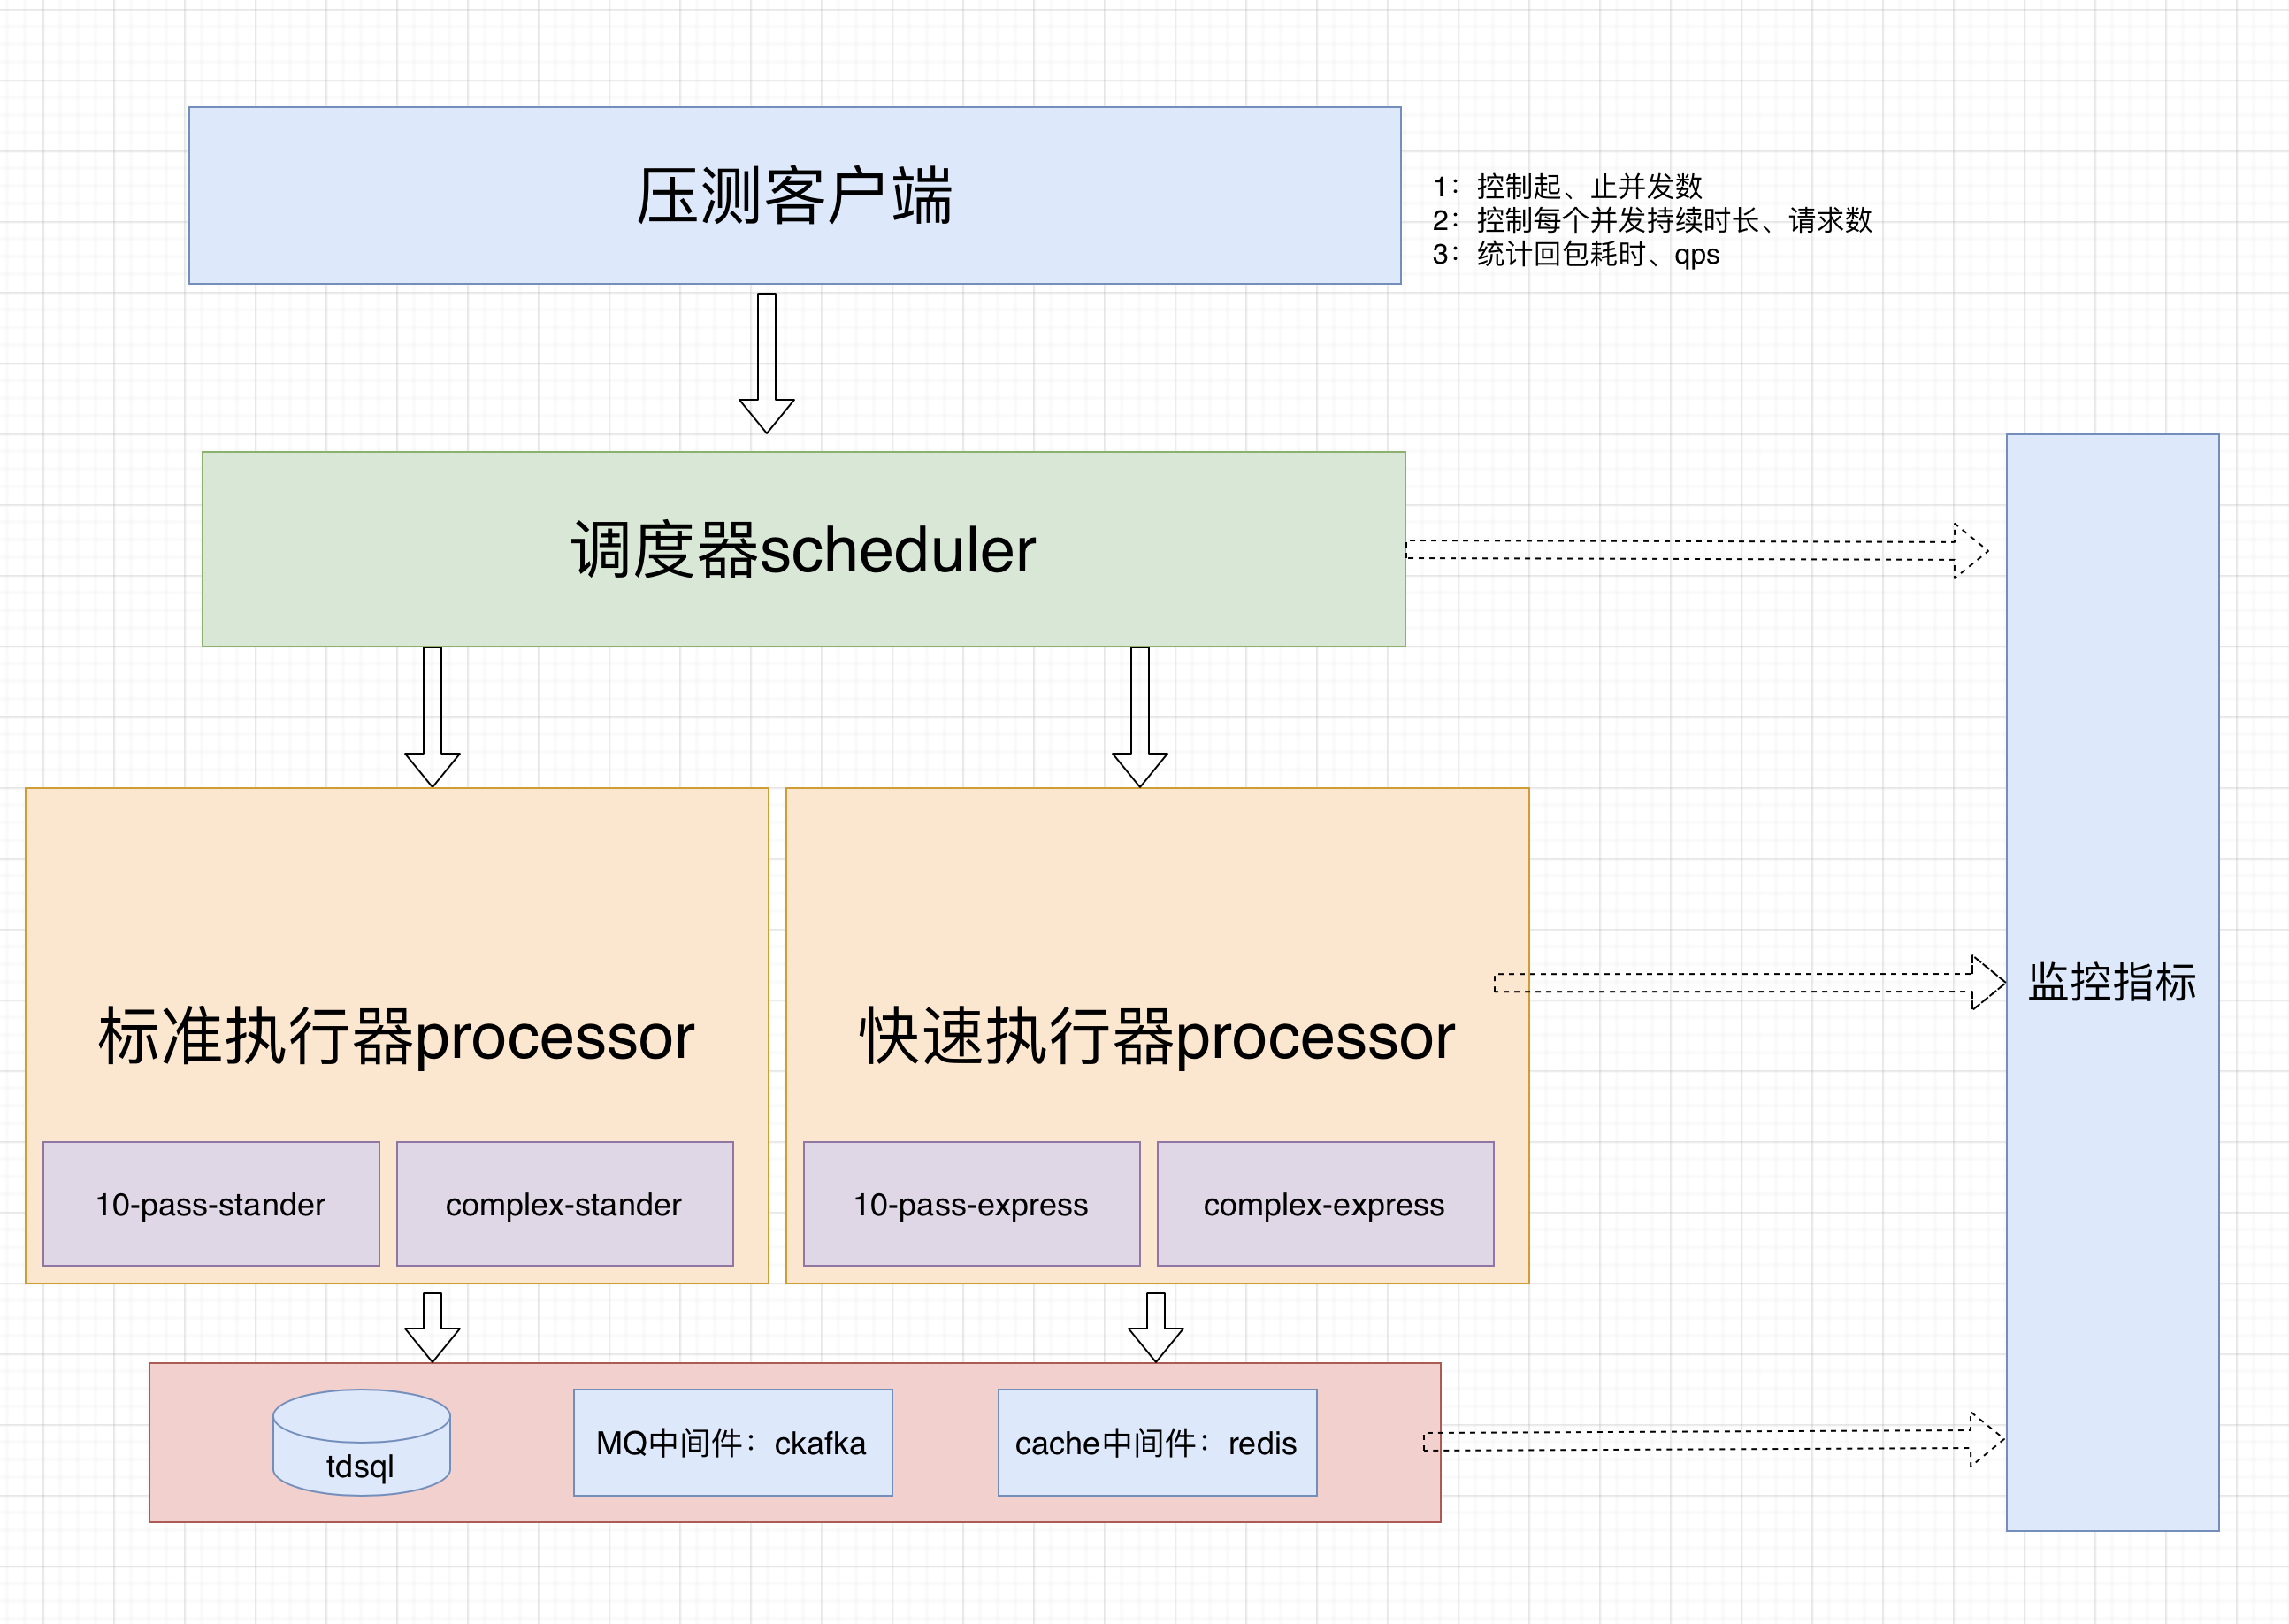
\includegraphics[width=0.9\textwidth]{press-test-2.png}
    \caption{6-3-1}
    \label{fig:6-1-2}
    \note{压测计划2}
\end{figure}

功能测试部分,通过自动化的接口测试,来保证每一次迭代上线的质量。沿用Go SDK自带的Test包,将所有发布的接口分别编写Test函数,再编写一个统一的测试
入口函数TestAll,该函数主要完成如下任务:
\begin{enumerate}
    \item 初始化构建测试数据库
    \item 读入测试用例
    \item 执行接口测试
    \item 输出测试结果
\end{enumerate}

测试数据库选用sqlite3,初始化使用migration-go, 进行数据库创建,使用go-xorm进行数据库操作(与业务DAO层保持一致)。测试用例使用JSON格式描述,
需要包含接口的输入参数,接口的预期输出。由于用例是JSON,因此断言部分主要使用jsonassert结合govaluate第三方包完成。

压力测试部分, 通过在搭建的微服务集群中创建一个容器,用于执行压力测试。


\section{功能性测试}
根据需求分析,需要测试的功能如下:

\subsection{工作流管理}

涉及的接口:

POST /v1/template/CreateTemplate

1.request.json:

\{

"TemplateName": "test",

"Description": "test",

"TemplateType": "EXPRESS",

%"Definition": "{\n\t\"Comment\": \"使用Pass节点演示hello world示例\",\n\t\"StartAt\": \"Hello\",\n\t\"States\": {\n\t\t\"Hello\": {\n\t\t\t\"Type\": \"Pass\",\n\t\t\t\"Comment\": \"传递\",\n\t\t\t\"Next\": \"World\"\n\t\t},\n\t\t\"World\": {\n\t\t\t\"Type\": \"Pass\",\n\t\t\t\"Comment\": \"传递\",\n\t\t\t\"End\": true\n\t\t}\n\t}\n}",

"TemplateStatus": "",

"UiConfig": ""

\}

1.response.json:

\{

"TemplateId": "\@exists()"

\}


POST /v1/template/ModifyTemplate

1.request.json:

\{

"TemplateId"          : "tpl-b8og5x47",

"TemplateName"        : "测试改名",

"Description"         : "测试修改描述",

%"Definition"          : "{\"Comment\":\"测试修改工作流\",\"StartAt\":\"Hello\",\"States\":{\"Hello\":{\"Type\":\"Pass\",\"Comment\":\"传递\",\"Next\":\"World\"},\"World\":{\"Type\":\"Pass\",\"Comment\":\"传递\",\"End\":true}}}",

"TemplateStatus"      : "PUBLISHED",

"UiConfig"            : ""

\}

1.response.json:

\{

    "Msg": "\@exists()"

    "ModifyTime": "\@exists()"

\}

POST /v1/template/DeleteTemplate

1.request.json:

\{

    "TemplateId": "\@exists()"

\}

1.response.json:

\{

    "Msg": "\@exists()"

    "DeleteTime": "\@exists()"

\}


POST /v1/template/CreateFlowService

1.request.json:

\{

"FlowServiceName"        : "testFlow1443",

"FlowServiceChineseName" : "测试工作流",

%"Definition"             : "{\"Comment\":\"使用Pass节点演示hello world示例\",\"StartAt\":\"Hello\",\"States\":{\"Hello\":{\"Type\":\"Pass\",\"Comment\":\"传递\",\"Next\":\"World\"},\"World\":{\"Type\":\"Pass\",\"Comment\":\"传递\",\"End\":true}}}",

"IsNewRole"              : false,

"Type"                   : "EXPRESS",

"RoleResource"           : "qrn:qcs:asw:ap-guangzhou:1301845006:http:json:flowmachine:test\_one:xqb4fdd1",

"Description"            : "description string",

"EnableCLS"              : false,

"Input"                  : ""

\}

1.response.json:

\{

"FlowServiceResource"   : "\@exists()",

"CreateDate"            : "\@exists()"

\}



POST /v1/template/ModifyFlowService

1.request.json:\{

    "FlowServiceResource"   : "qrn:qcs:asw:ap-guangzhou:1259772248:http:json:flowmachine:zzz:c139dqb7",

%"Definition"            : "{\"Comment\":\"使用Pass节点演示hello world示例\",\"StartAt\":\"Hello\",\"States\":{\"Hello\":{\"Type\":\"Pass\",\"Comment\":\"传递\",\"Next\":\"World\"},\"World\":{\"Type\":\"Pass\",\"Comment\":\"传递\",\"End\":true}}}",

    "FlowServiceName"       :  "zzz",

    "FlowServiceChineseName":  "测试改中文名",

    "IsNewRole"             :  false,

    "Type"                  :  "STANDARD",

    "RoleResource"          :  "qcs::cam::uin/100011023428:roleName/zzz\_1304034199\_c139dk16",

    "Description"           :  "测试修改描述",

    "EnableCLS"             :  false

\}

1.response.json:

\{

"FlowServiceResource": "\@notEmpty()",

"UpdateDate": "\@notEmpty()"

\}

POST /v1/template/DeleteFlowService

1.request.json:

\{

    "TemplateId": "\@exists()"

\}


1.response.json:

\{

    "Msg": "\@exists()"

    "DeleteTime": "\@exists()"

\}


\subsection{工作流执行}
POST /v1/scheduler/StartExecution

Parallel模式、Normal模式

1.request.json:

\{

"Input": "\@exists()"

"Name": "\@notEmpty()"

\}


1.response.json:

\{

"ExecutionQrn": "\@notEmpty()"

\}



GET /v1/processor/GetTaskStatus

1.request.json:

\{

"TaskIds": "\@exists()"

\}


1.response.json:

\{

"TaskStatus": "\@exists()"

"Error": "\@notExists()"

\}

POST /v1/processor/SubmitCmd

1.request.json:

\{

\}

1.response.json:

\{

\}

\subsection{查询工作流列表}
GET /v1/template/DescribeTemplates

1.request.json:

\{

"TemplateIds": [
"tpl-b8og5x47",
"tpl-bcquf84m"
],

"Offset": 0,

"Limit": 10,

"Filters": [\{

    "Name": "TemplateType",

    "Values": ["QUICK\_START"]
\}]

\}


1.response.json:

\{

\}

GET /v1/template/DescribeFlowServices

1.request.json:

\{

"Offset": 0,

"Limit": 10,

"Filters": [\{

"Name": "Type",

"Value": "EXPRESS"

\}]

\}

1.response.json:

\{

"TotalCount": "\@exists()",

"FlowServiceSet": "\@exists()"

\}

\subsection{查询工作流详情}
GET /v1/template/DescribeFlowServiceDetail


1.request.json:
\{
"FlowServiceResource": "qrn:qcs:asw:ap-guangzhou:1259772248:http:json:flowmachine:zzz:c139dqb7"
\}
1.response.json:
\{
"FlowServiceName"        :  "\@notEmpty()",
"Status"                 :  "\@notEmpty()",
"Definition"             :  "\@notEmpty()",
"RoleResource"           :  "\@notEmpty()",
"Type"                   :  "\@notEmpty()",
"CreateDate"             :  "\@notEmpty()",
"Description"            :  "\@notEmpty()",
"FlowServiceChineseName" :  "\@exists()"
\}

\subsection{工作流应用模板部署}
GET /v1/template/DescribeTemplateResources
1.request.json:
\{
"TemplateId": "tpl-c59aj3jz"
\}
1.response.json:
\{
"Resources": "\@exists()"
\}

GET /v1/template/DescribeDeployResults

1.request.json:
\{
"TemplateId": "tpl-c59aj3jz",
"ExecutionQRN": "qrn:qcs:asw:ap-guangzhou:1300746878:execution:bu5op4dq:bu5uui21bu5uui22-bu5uui23-bu5uui24-bu5uui25"
\}

1.response.json:
\{
"DeployResults": "\@exists()",
"MachineQrn": "\@len()\>30"
\}

POST /v1/scheduler/StartDeploy

\subsection{工作流应用模板查询}

GET /v1/template/DescribeApplicationTemplates
1.request.json:
\{
\}

1.response.json:
\{
"Templates": "\@exists()"
\}

\subsection{权限管理}

POST /v1/auth/CreateUserStatus
1.request.json:
\{
"uid": "123456"
\}

1.response.json:
\{
\}
GET /v1/auth/DescribeUserStatus
1.request.json:
\{
\}

1.response.json:
\{
"IsNewUser": "\@exists()"
"GrantUrl": "\@exists()"
"LogFlagBit": "\@exists()"
\}

POST /v1/auth/DescribeToken
1.request.json:
\{
"RoleQRN": "\@notEmpty()"
"Region": "\@notEmpty()"
\}

1.response.json:
\{
"SecretId: "\@notEmpty()"
"SecretKey: "\@notEmpty()"
"Token: "\@exists()"
"ExpiredTime: "\@exists()"
\}

%测试用例设计:
%curl localhost:59901 -d '{
%"Action":"CreateFlowService",
%"AppID":251197975,
%"Uin":"100000085051",
%"SubAccountUin":"100000085051",
%"Region": "ap-guangzhou",
%"Version": "2020-07-22",
%%"Definition": "{\n  \"Comment\": \"A Hello World example of the Tencent ASW States Language using Pass states\",\n  \"StartAt\": \"Hello\",\n  \"States\": {\n    \"Hello\": {\n      \"Type\": \"Pass\",\n      \"Comment\": \"传递\",\n      \"Next\": \"World\"\n    },\n    \"World\": {\n      \"Type\": \"Pass\",\n      \"Comment\": \"传递\",\n      \"End\": true\n    }\n  }\n}",
%"FlowServiceName": "test-create-with-cls",
%"FlowServiceChineseName": "",
%"IsNewRole": false,
%"Type": "EXPRESS",
%%"RoleResource": "qcs::cam::uin/100000085051:roleName/ASW_QCSLinkedRoleInCLS",
%"EnableCLS":true
%}'
%
%curl localhost:59901 -d '{
%"Action":"ModifyFlowService",
%"AppID":251197975,
%"Region":"ap-guangzhou",
%"Uin":"251197975",
%"Version": "2020-07-22",
%"FlowServiceName": "test123",
%"FlowServiceChineseName": "1",
%"FlowServiceResource": "qrn:qcs:asw:ap-guangzhou:251197975:http:json:flowmachine:test123:chvuuxcd",
%"IsNewRole": false,
%%"Definition": "{\n  \"Comment\": \"A Hello World example of the Tencent ASW States Language using Pass states\",\n  \"StartAt\": \"Hello\",\n  \"States\": {\n    \"Hello\": {\n      \"Type\": \"Pass\",\n      \"Comment\": \"传递\",\n      \"Next\": \"World\"\n    },\n    \"World\": {\n      \"Type\": \"Pass\",\n      \"Comment\": \"传递\",\n      \"End\": true\n    }\n  }\n}",
%%"RoleResource": "qcs::cam::uin/100000085134:roleName/ASW_QCSLinkedRoleInCLS",
%"Description": "",
%"Type": "STANDARD",
%"EnableCLS":true}'
%
%
%
%curl localhost:59901 -d '{
%"Action":"DescribeFlowServiceDetail",
%"AppID":251197975,
%"Uin":"100000085051",
%"SubAccountUin":"100000085051",
%"FlowServiceResource":"qrn:qcs:asw:ap-guangzhou:251197975:http:json:flowmachine:test-create-with-cls:chvzhk0b"
%}'
%
%获取用户状态
%curl localhost:32124 -d '{"Action":"DescribeUserStatus", "Region":"ap-guangzhou", "Uin":"100011023428"}'
%
%应用模板功能
%curl localhost:59901 -d '{"Action":"DescribeApplicationTemplates", "Region":"ap-guangzhou", "Uin":"100000085051"}'
%curl localhost:59901 -d '{"Action":"DescribeTemplateResources", "Region":"ap-guangzhou", "Uin":"100000085051", "TemplateId": "tpl-c59aj3jz"}'
%
%curl localhost:59901 -d '{
%"Action":"DescribeDeployResults",
%"AppID":251197975,
%"Version": "2020-07-22",
%"Uin":"100000085051",
%"SubAccountUin":"100000085051",
%"TemplateId": "tpl-c59aj3jz",
%"ExecutionQRN": "qrn:qcs:asw:ap-guangzhou:251009330:execution:test:lyt"
%}'


\section{非功能性测试}

根据需求分析的非功能性功能部分,需要测试的部分如下:

\subsection{服务合并}
111
%curl localhost:59901 -d '{"Action":"DescribeComponentTree"}'
%
%curl localhost:59901 -d '{"Action":"DescribeComponents"}'
%
%curl localhost:59901 -d '{"Action":"CreateFlowServiceComponent", "Region": "ap-guangzhou", "uin": "100011023428", "subAccountUin":"100011023428", "appid": 1259772248, "FlowServiceId": "asr-checkAsrJob", "ReturnCode": "200", "ServiceName": "test123", "ChineseName": "测试", "Name": "test123"}'
%
%curl localhost:59901 -d '{"Action":"GetComponentDetail", "ComponentResource": "qrn:qcs:asw:ap-guangzhou:1259772248:http:json:flowmachine:test123:test123"}'
%
%curl localhost:59901 -d '{"Action": "DeleteFlowServiceComponent", "Region": "ap-guangzhou", "uin": "100011023428", "subAccountUin":"100011023428", "appid": 1259772248, "ComponentResource": "qrn:qcs:asw:ap-guangzhou:1259772248:http:json:flowmachine:test123:test123"}'
%

\subsection{预测执行}

预测器服务
POST /v1/predict/Predict
POST /v1/predict/ExecutionRecord

\subsection{动态负载探活}
POST /v1/processor/Healthy

\subsection{内存管理优化}
压测,火焰图?

\subsubsection{服务降级、熔断策略}


\subsection{自动化测试能力建设}
go test TestALl.go


\subsection{日志巡检}

参数:threshold,超过该值的日志不进行重复输出。不填默认为10
python3 search\_error.py 10

\begin{figure}
    \centering
    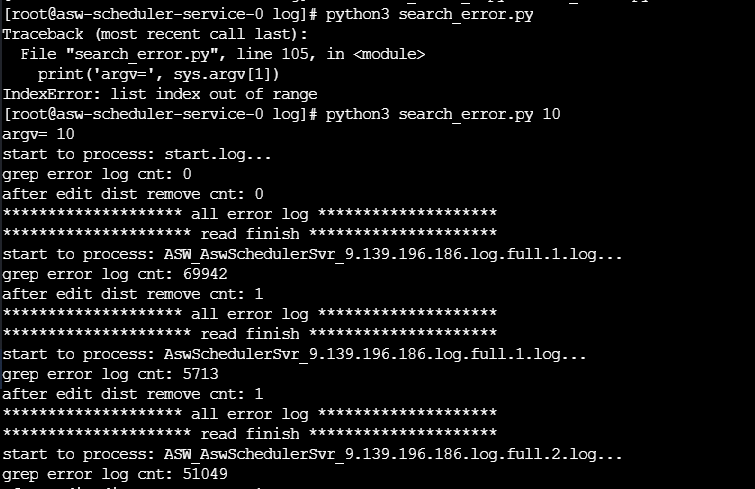
\includegraphics[width=0.6\textwidth]{log-1.png}
    \caption{巡检1}
    \label{fig:6-4-1}
    \note{巡检1}
\end{figure}

\begin{figure}
    \centering
    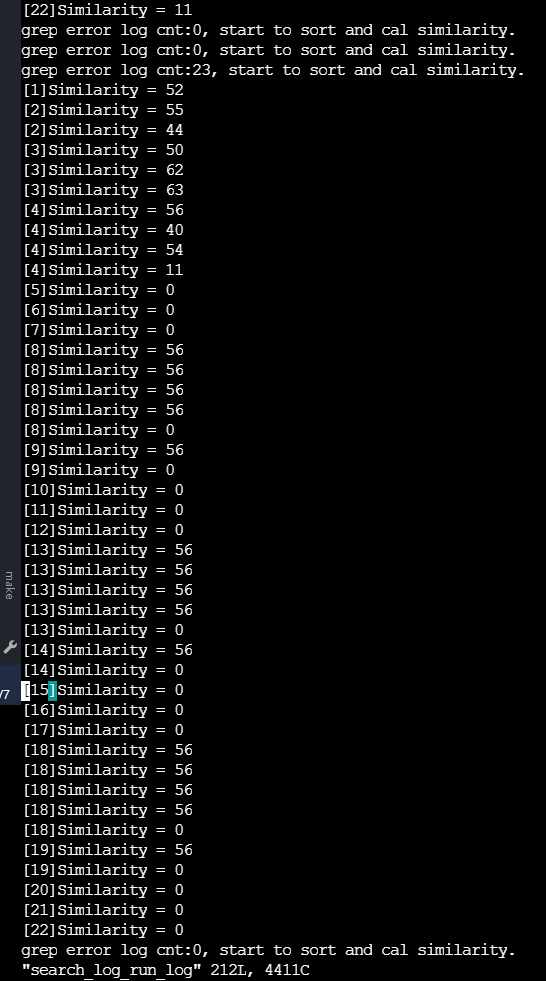
\includegraphics[width=1.0\textwidth]{log-2.png}
    \caption{巡检2}
    \label{fig:6-4-2}
    \note{巡检2}
\end{figure}

\begin{figure}
    \centering
    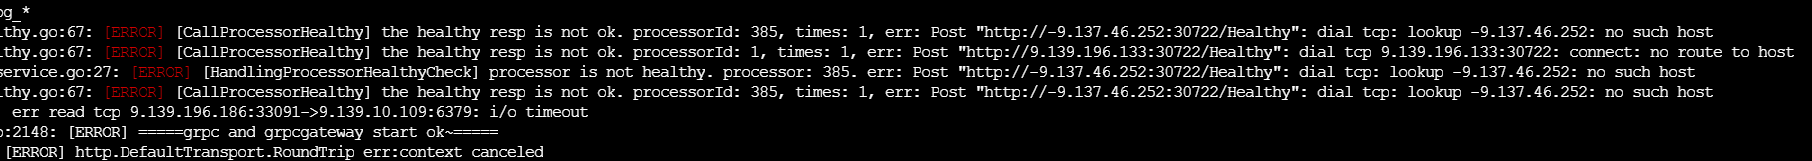
\includegraphics[width=1.5\textwidth]{log-3.png}
    \caption{巡检3}
    \label{fig:6-4-3}
    \note{巡检3}
\end{figure}

\subsection{缓存淘汰策略}
ZRANGE ES\_\{Machine\_Qrn\} -inf +inf
附图:

经过清理算法后,每个用户工作流只存储1000条历史执行数据。


\section{压力测试}


使用https://github.com/link1st/go-stress-testing开源项目作为压力测试工具。该项目是一个go 实现的压测工具,每个用户用一个协程的方
式模拟,最大限度的利用 CPU 资源。go-stress-testing-amd -c 1 -n 100 -u localhost:8000

新建shell脚本,用于执行命令 ./go-stress-testing-amd -c $cur_con -n $req\_num -p \$curl\_file

在容器控制台执行sh press\_test.sh 100 100000 curl/stress-test-1.sh

参数\$1, \$2, \$3含义是设置并发协程数为100,请求量为100000,执行curl/stress-test-1.sh脚本里的curl请求语句(需提前写好TODO)。

对StartExecution、SubmitCmd两个接口分别进行压力测试。前者对全链路涉及的服务都会覆盖,反应整个流程的性能好坏;后者仅是链路中的关键步骤,反应
了容器执行的速度性能。


对SubmitCmd接口压测,并发数:120 请求数:20000000
POST /v1/processor/SubmitCmd

\begin{figure}[H]
    \centering
    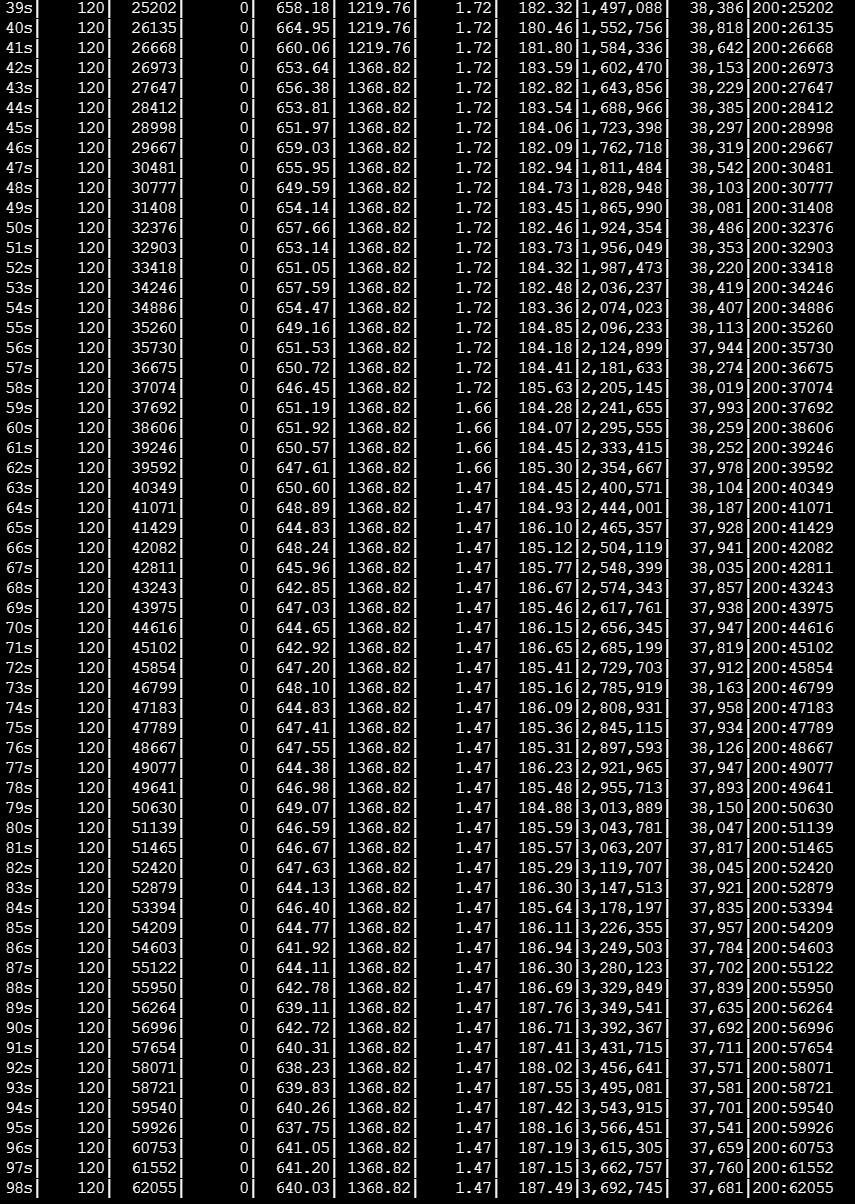
\includegraphics[width=0.9\textwidth]{6-3-1.jpg}
    \caption{6-3-1}
    \label{fig:6-3-1}
    \note{压测过程}
\end{figure}

\begin{figure}[H]
    \centering
    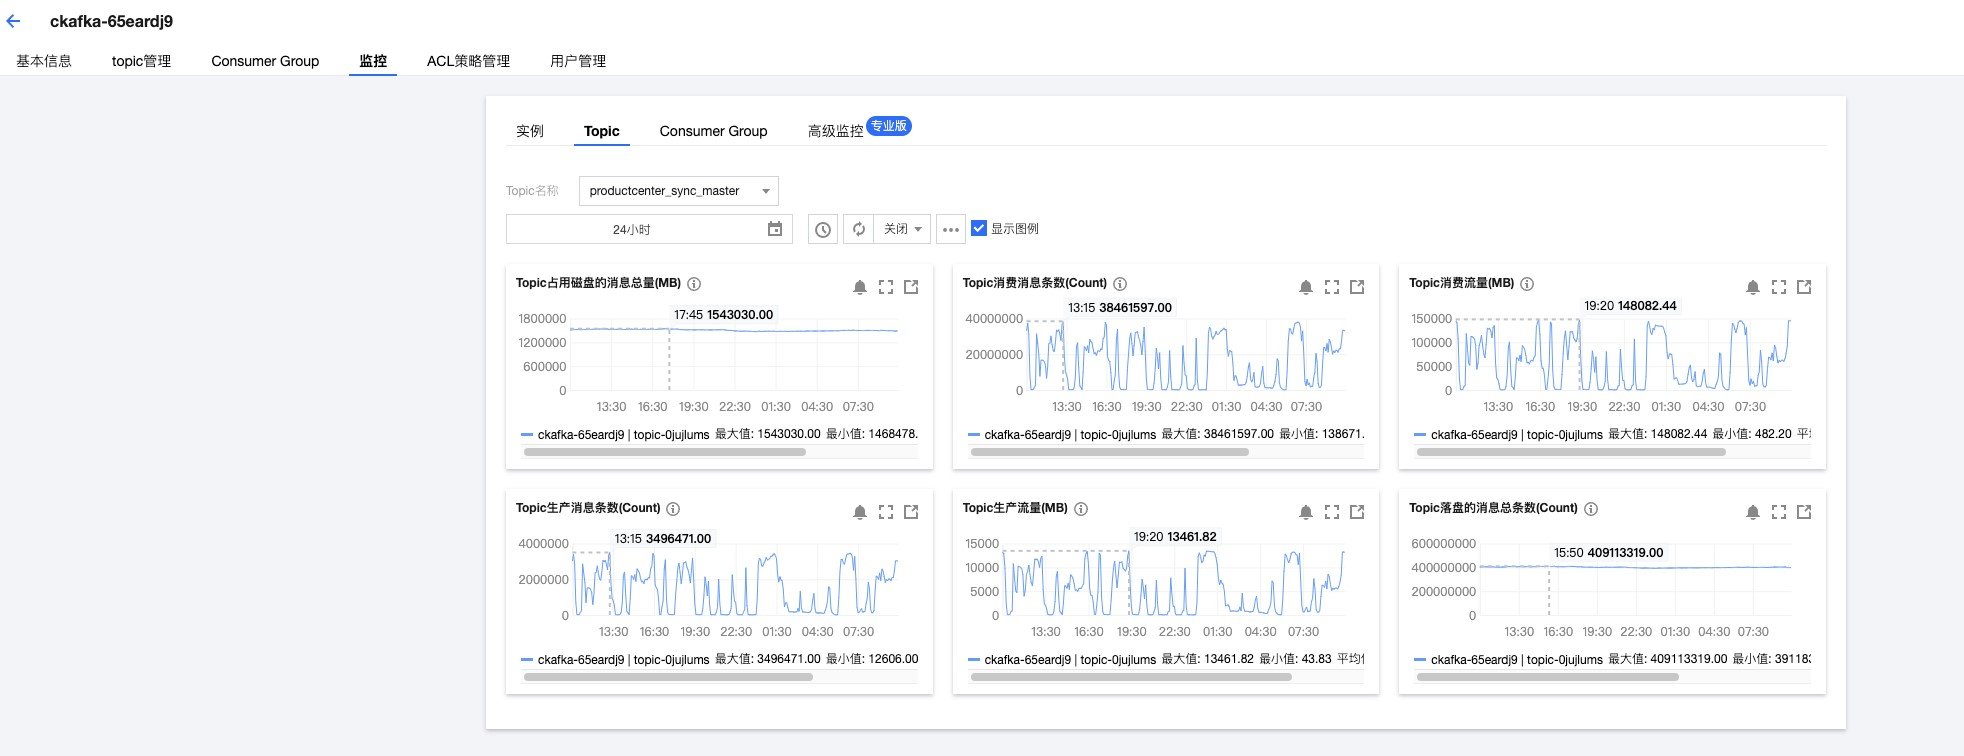
\includegraphics[width=0.9\textwidth]{6-3-2.jpg}
    \caption{6-3-2}
    \label{fig:6-3-2}
    \note{监控状态}
\end{figure}

对StartExecution接口的Normal模式压测,并发数:120 请求数:20000000
POST /v1/scheduler/StartExecution

对StartExecution接口的Parallel模式压测,并发数:120 请求数:20000000
POST /v1/scheduler/StartExecution


\section{本章小结}

本章阐述了对系统做了全方位的测试,包括功能性测试和功能性测试,确保了系统的设计功能的完备和可用,以及模拟大流量场景下系统表现的情况。
对系统整体的性能指标有了量化后的数据图表可供进一步分析,为性能优化的方案设计提供重要的参考价值。